\section{Strength of materials - Beams}
A straigth horizontal beam with Young modulus $E$, length $L$,
square cross-section $S$, bending inertia $I$,
is free at its extremity, loaded only by a vertical force $F$
at its mid-length and clamped at the origin.
A drawing of the problem is shown in Figure~\ref{fig:beam_1}.
Let $u(x)$ the vertical displacement.

We know that
\[ u''(x) = \frac{M(x)}{E I} \]
where $M(x)$ is the bending moment,
which we found few lines down from here
when computing the shear force and bending moment diagrams.

From equations~\myref{eq:beam_M_cut1} and~\myref{eq:beam_M_cut2},
we have
\begin{enumerate}
  \item for $x\in[0,L/2]$
  \begin{align*}
    u''(x) &= \frac{1}{E  I}\, F (x - \frac{L}{2}) \\
    u'(x) &= \frac{1}{E  I}\left(F\frac{x^2}{2} - \frac{L}{2} x \right)
    + C_1 \\
    u(x) &= \frac{1}{E  I}\left(F\frac{x^3}{6} - \frac{L}{4} x^2 \right)
    + C_1 x + C_2
  \end{align*}
  \item for $x\in[L/2,L]$
  \begin{align*}
    u''(x) &= 0 \\
    u'(x) &= C_3 \\
    u(x) &= C_3 x + C_4
  \end{align*}
\end{enumerate}

The known boundary conditions are the following
\begin{itemize}
\renewcommand\labelitemi{$\bullet$}
  \item $u(0) = 0$ as the beam doesn't experience
  any deflection at the wall,
  \item $u'(0) = 0$ as the beam is assumed 
  to be horizontal at the wall,
  \item $u''(L) = 0$ as we assume no bending moment
  at the free end of the beam,
  \item $u'''(L) = 0$ as we assume no shearing force
  acting at the free end of the beam.
\end{itemize}

Using these conditions we can easily show that
\[ C_i = 0 \qquad \forall i \in [1,4] \]

%Finally,
%\[
%  u(x) = 
%  \left\{ 
%    \begin{array}{rcl}
%      \frac{1}{E  I}\left(F\frac{x^3}{6} 
%      - \frac{L}{4} x^2 \right) & \mbox{if} & x \in [0,L/2] \\ 
%      0 & \mbox{if} & x \in [L/2,L] \\
%    \end{array}
%  \right.
%\]

\begin{figure}[h]
  \begin{center}
    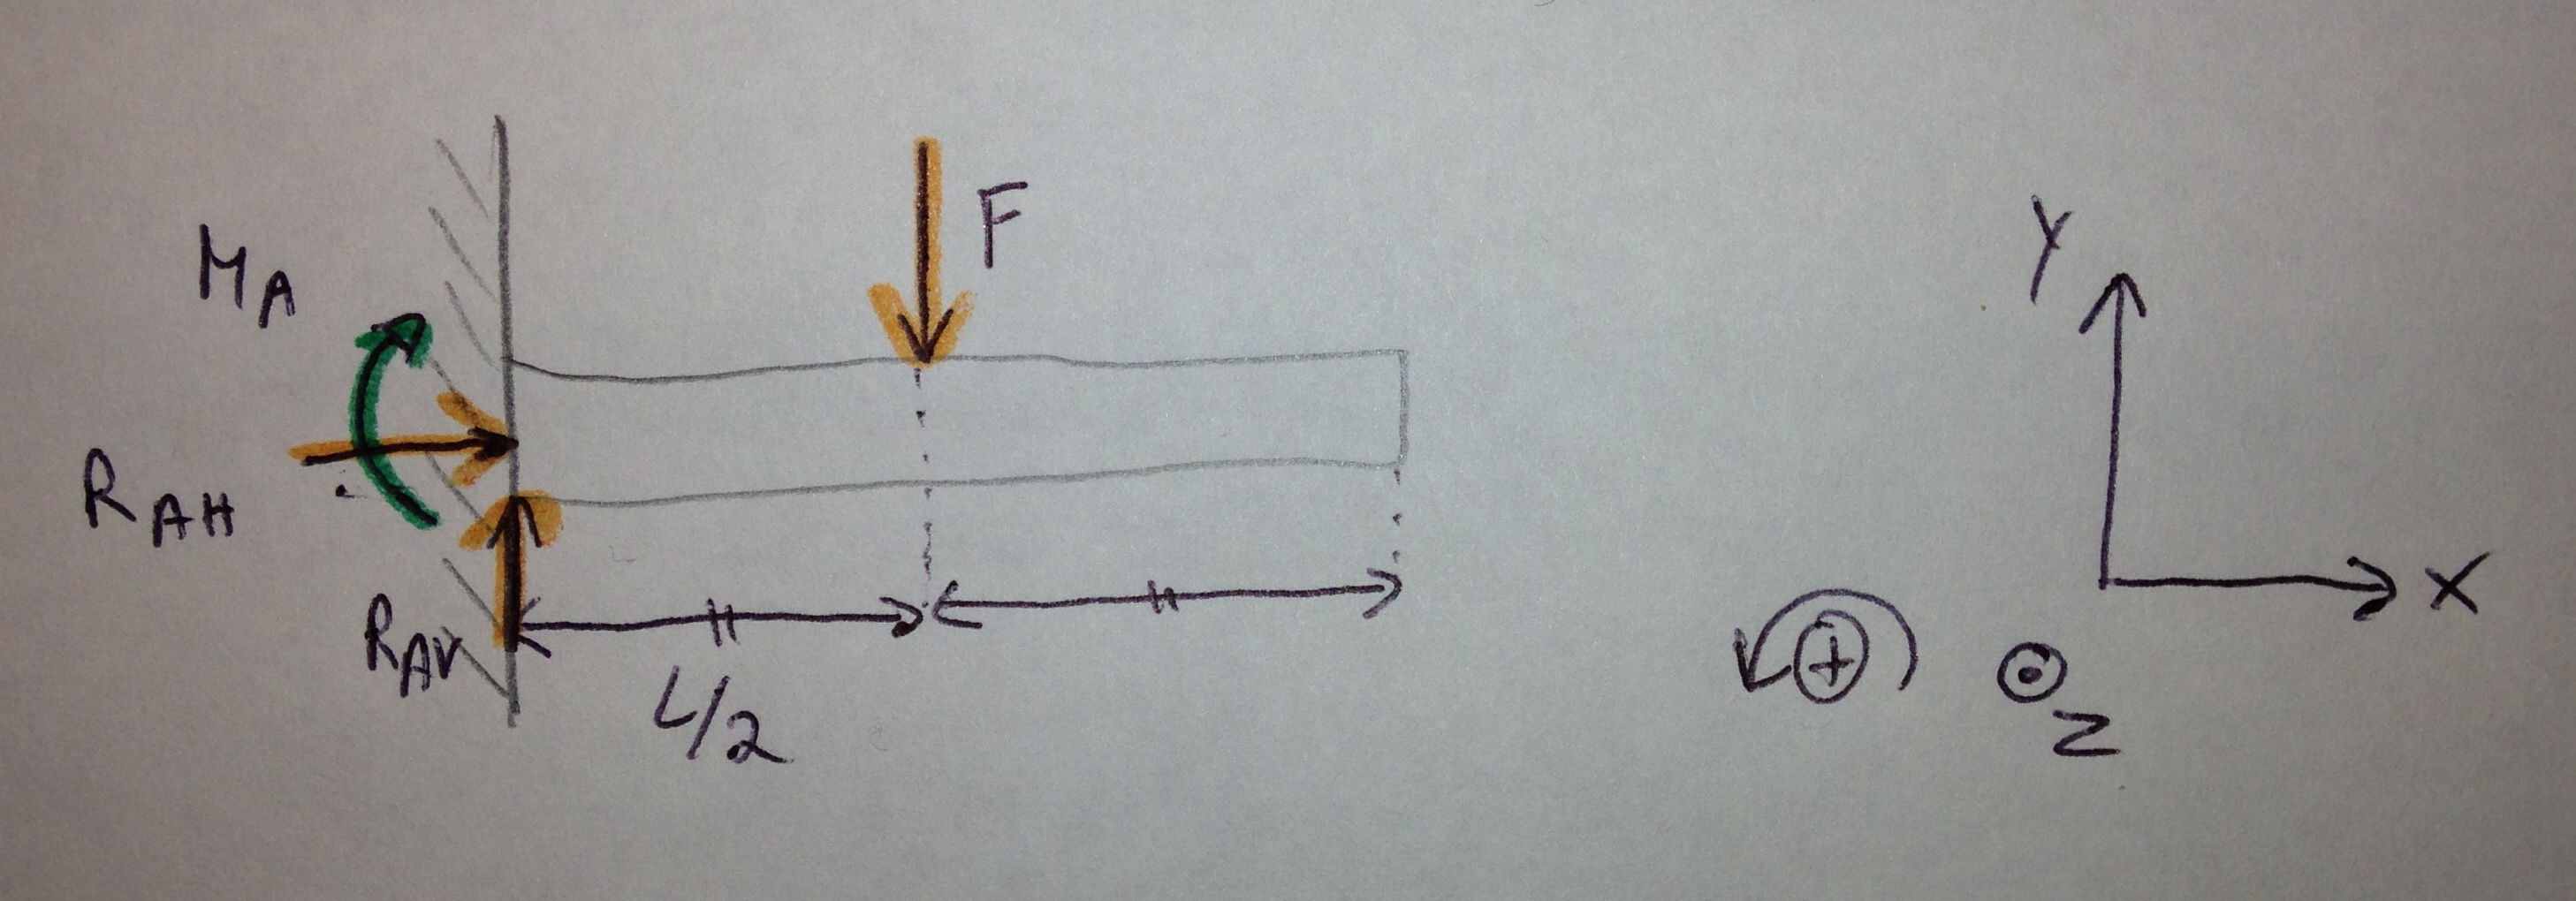
\includegraphics[scale=0.09]{beam1.jpg}
    \caption{General problem.}
    \label{fig:beam_1}
  \end{center}
\end{figure}

We are now going to find the \emph{shear force} $V(x)$
and the \emph{bending moment} $M(x)$ where $x$ varies between $[0,L]$.

First, we set the general conditions.
\begin{align*}
  \sum F = 0 &\iff R_{AV} - F = 0 \\
  &\iff R_{AV} = F \\
  \sum \tau = 0 &\iff -M_A - \frac{L}{2} F = 0 \\
  &\iff M_A = - \frac{L}{2} F
\end{align*}
Note that the torque is defined positive in the 
counter-clockwise direction, as seen in Figure~\ref{fig:beam_1}.

Now our goal will be to find $V$ and $M$ along the beam,
we will proceed by iterating the above step for each cut.
A cut is defined when a new force appears.
We define $x$ as being the distance of the cut from the origin.

Thus, we have for $x \in [0,L/2]$, shown in Figure~\ref{fig:beam_2}.
\begin{align}
  \sum F = 0 &\iff R_{AV} - V = 0 \nonumber \\
  &\iff T = F \label{eq:beam_V_cut1}\\
  \sum \tau = 0 &\iff -M_A - x\, V + M = 0 \nonumber \\
  &\iff M = F (x - L/2) \label{eq:beam_M_cut1}
\end{align}

\begin{figure}[h]
  \begin{center}
    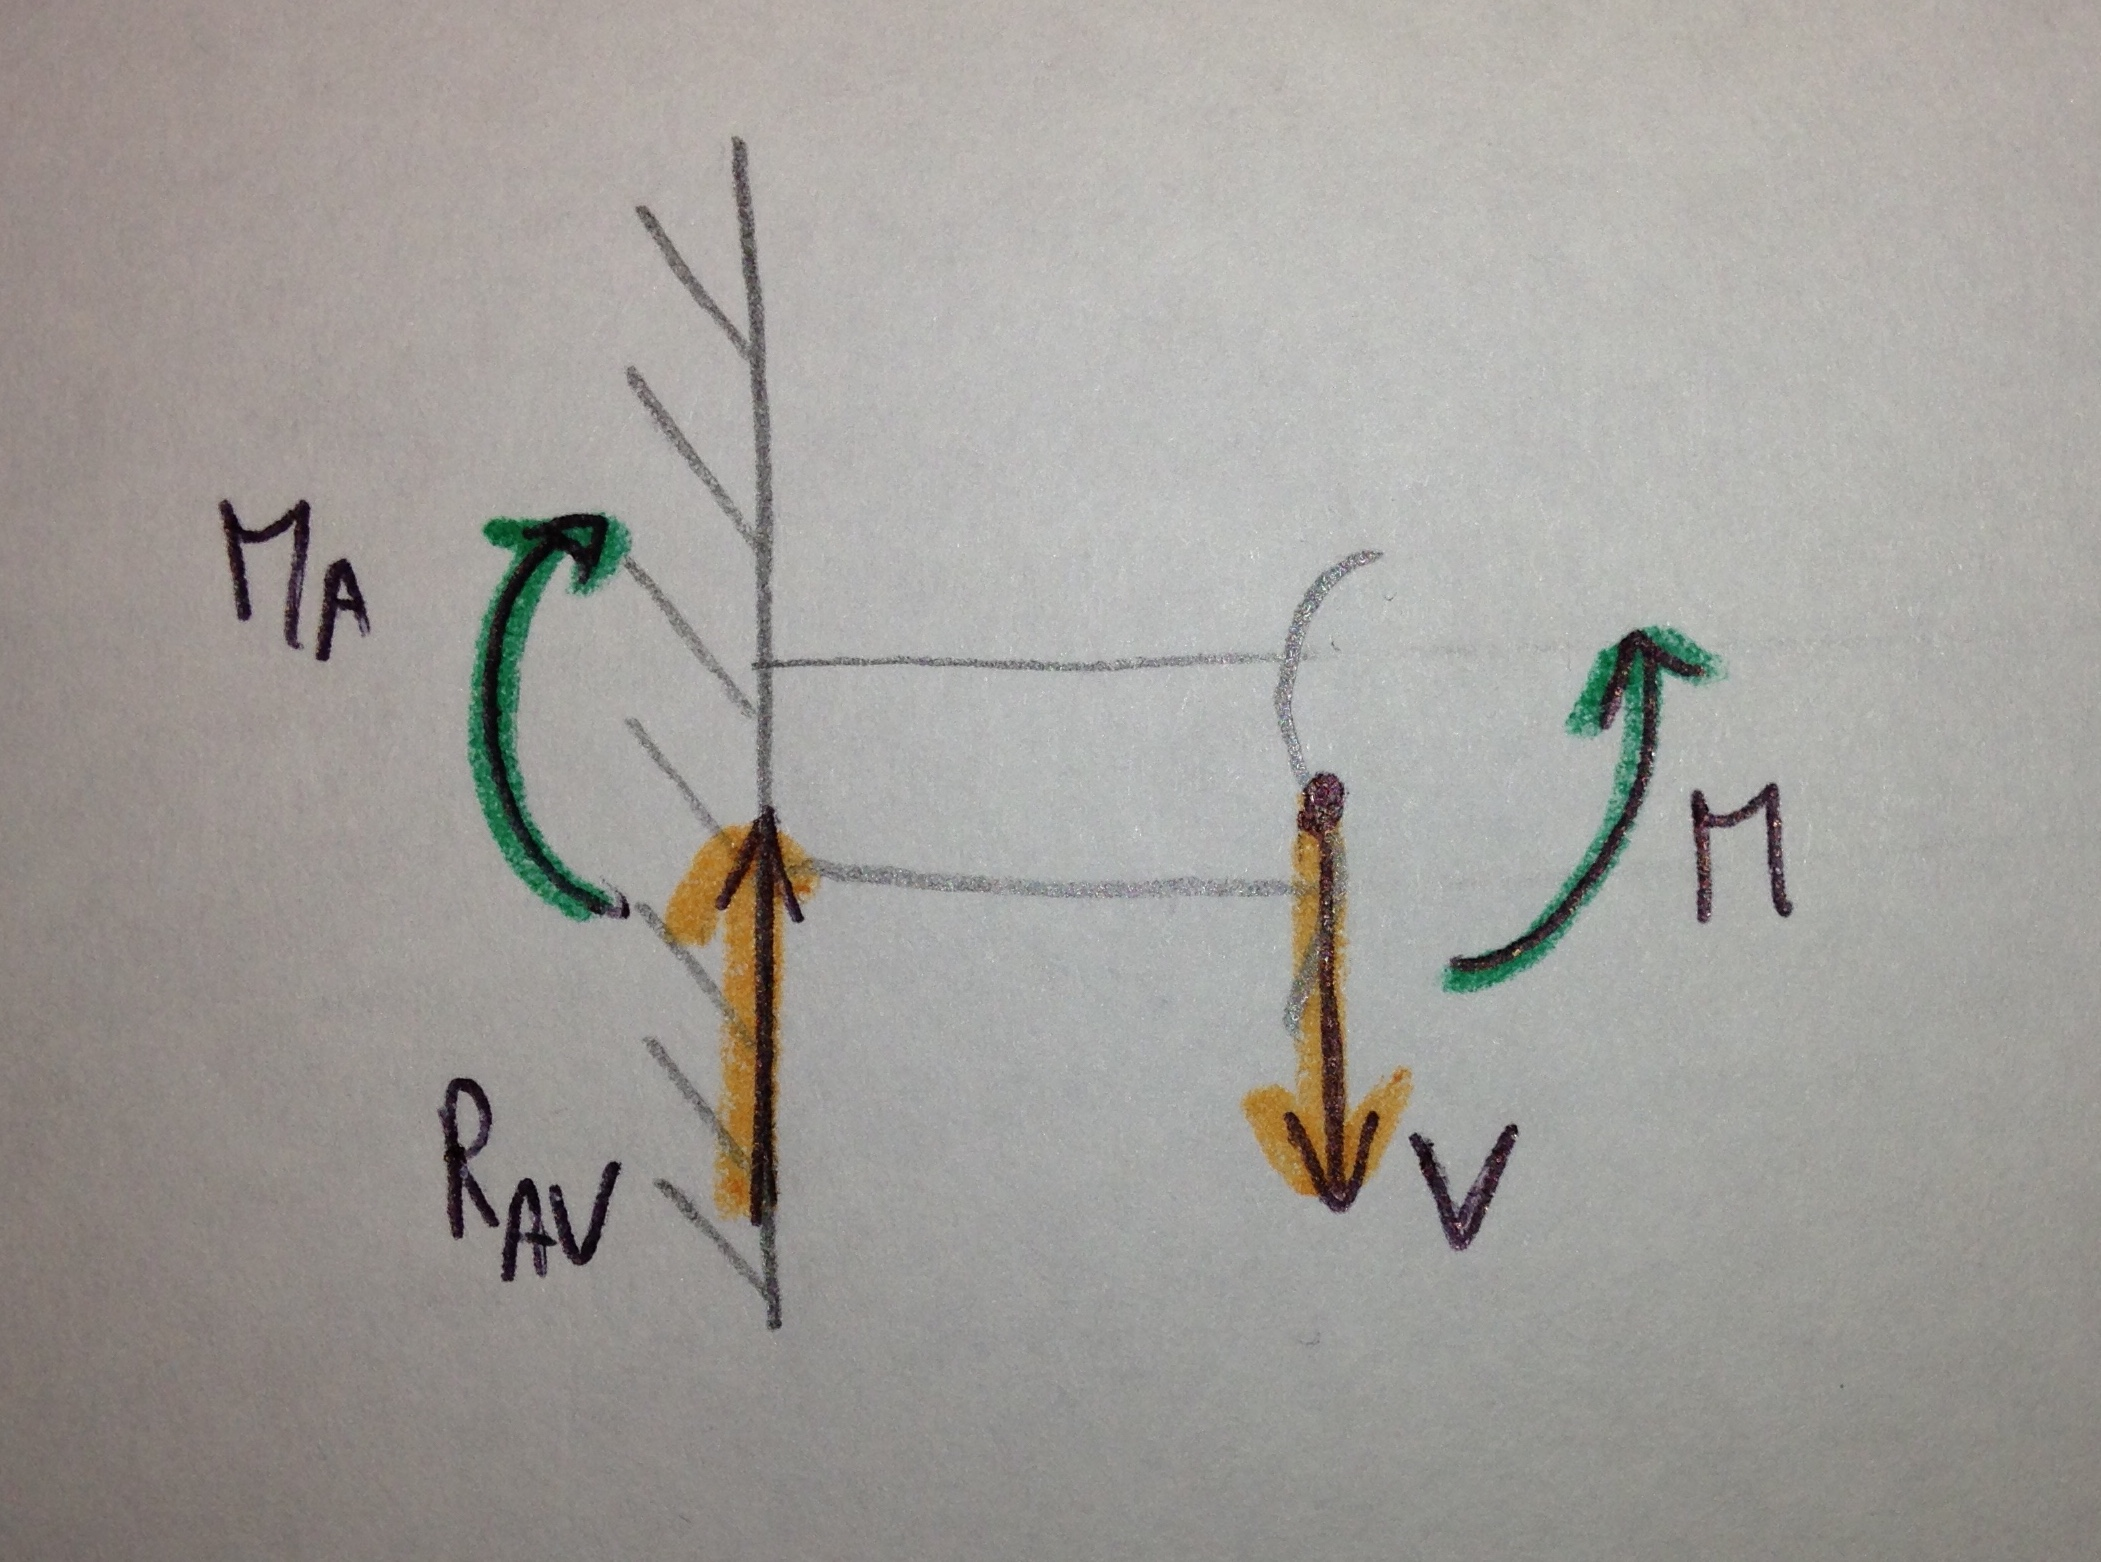
\includegraphics[scale=0.07]{beam2.jpg}
    \caption{First cut.}
    \label{fig:beam_2}
  \end{center}
\end{figure}

Then, for $x \in [L/2, L]$, shown in Figure~\ref{fig:beam_3}.
\begin{align}
  \sum F = 0 &\iff R_{AV} - F - V = 0 \nonumber \\
  &\iff V = 0 \label{eq:beam_V_cut2}\\
  \sum \tau = 0 &\iff -M_A -\frac{L}{2} F - x \, T + M = 0 \nonumber \\
  &\iff M = 0 \label{eq:beam_M_cut2}
\end{align}

\begin{figure}[h]
  \begin{center}
    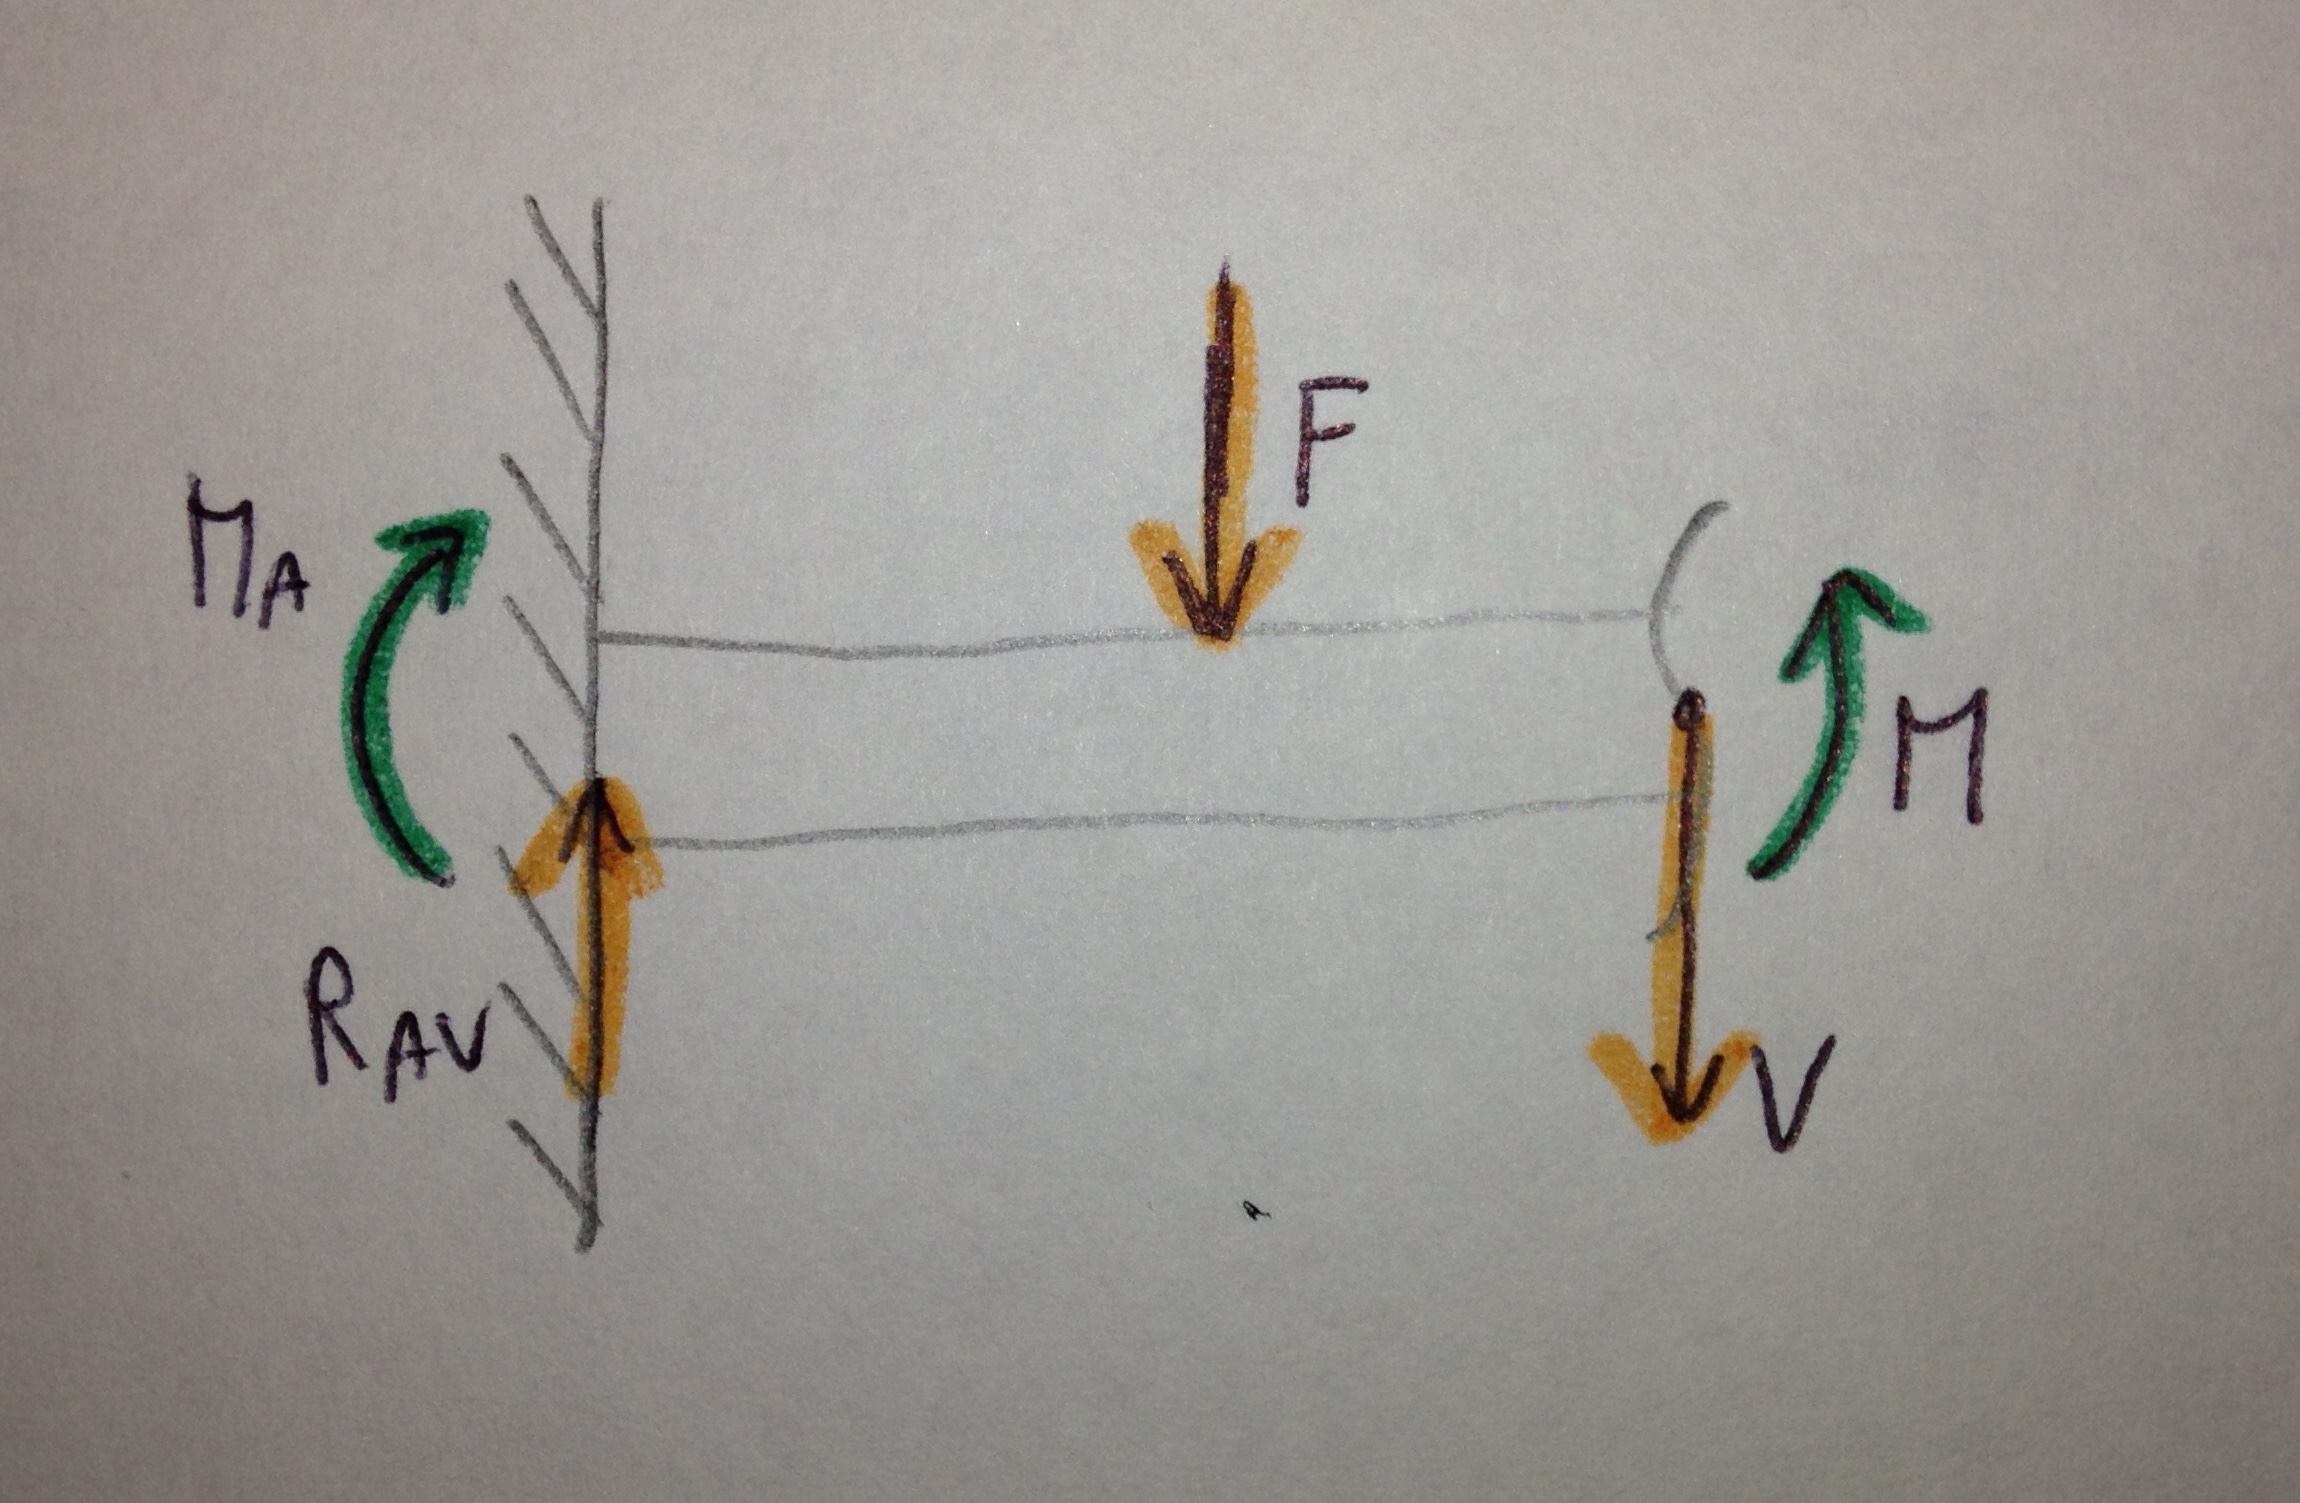
\includegraphics[scale=0.08]{beam3.jpg}
    \caption{Second cut.}
    \label{fig:beam_3}
  \end{center}
\end{figure}

Using equations~\myref{eq:beam_V_cut1} to~\myref{eq:beam_M_cut2},
we can draw the diagrams found in Figure~\ref{fig:beam_4}.
\begin{figure}[h]
  \begin{center}
    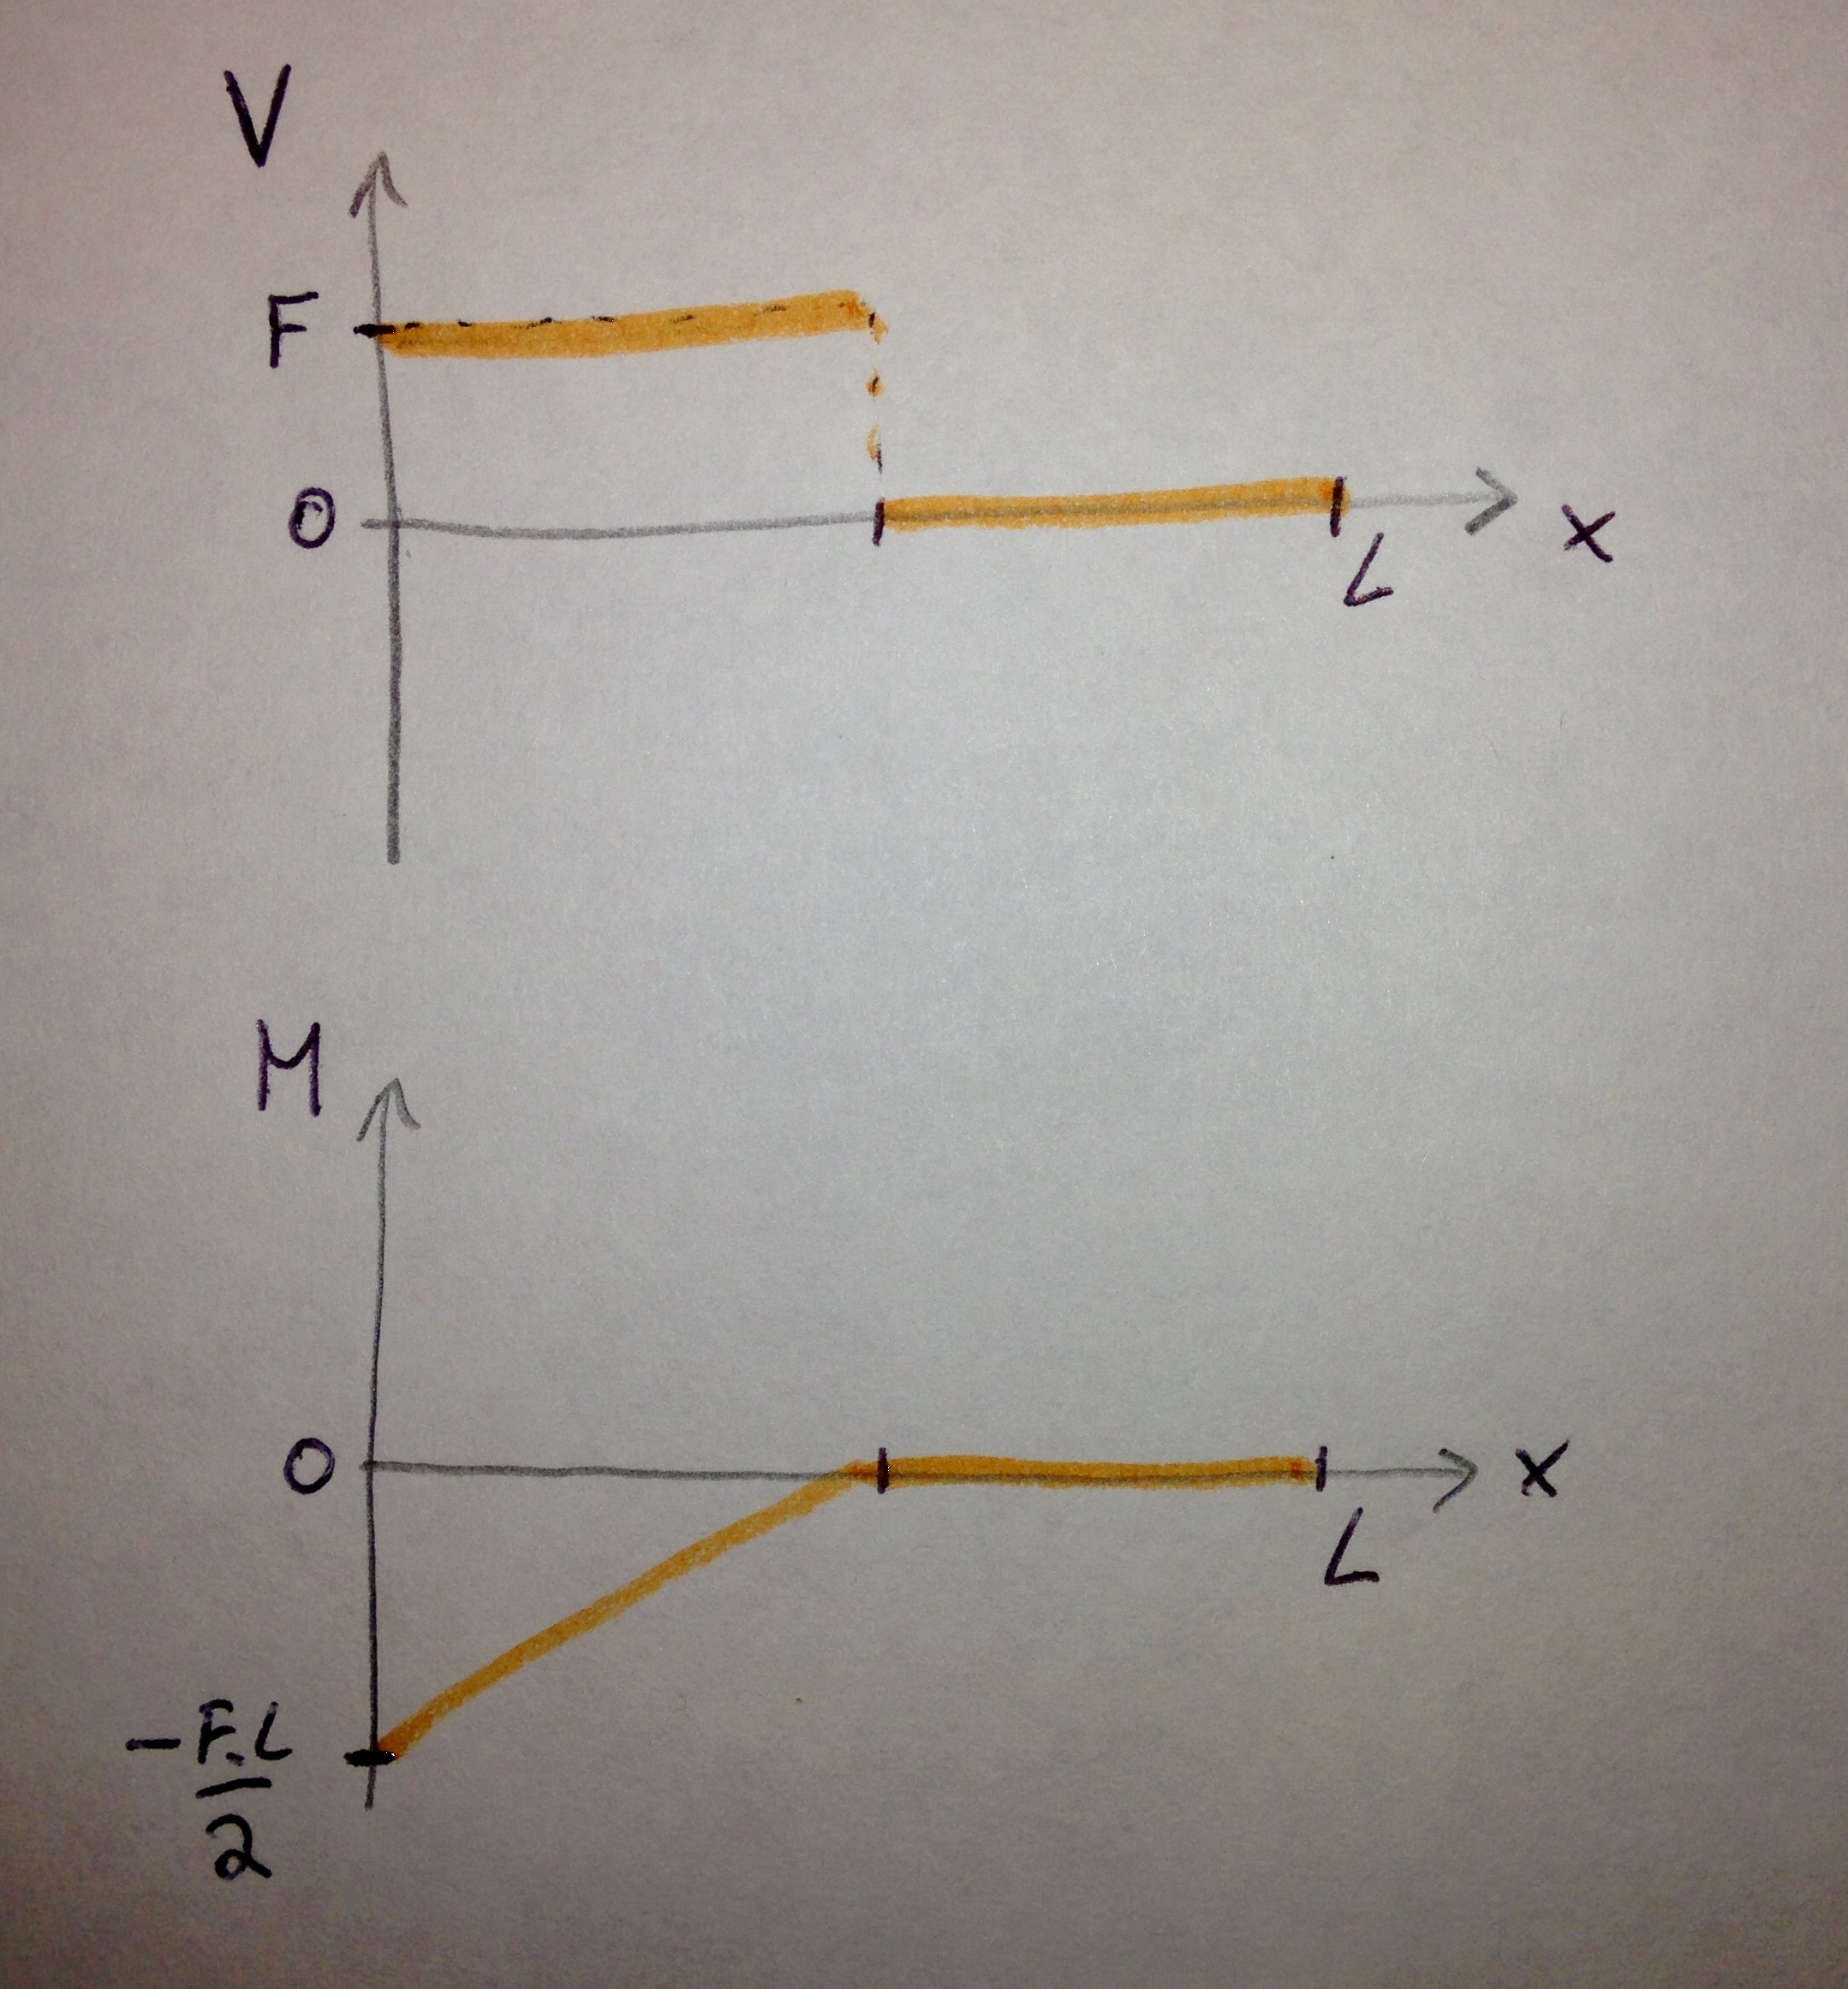
\includegraphics[scale=0.07]{beam4.jpg}
    \caption{Shear force $V$ diagram and bending moment $M$ diagram
    at the origin.}
    \label{fig:beam_4}
  \end{center}
\end{figure}